\part{Entwicklerhandbuch}

\chapter{Übersicht}
\chapter{Algorithmus}
\todo{hier muss erklärt werden wie der Algorithmus mit den Zählern funktioniert und ggf. warum das O(1) ist}
\chapter{Benutzeroberfläche}
\todo{hier muss erklärt werden wie ReactJS funktioniert und warum es die Performance verbessert}
Damit die aktiven Zustände hervorgehoben werden können, müssen sie eindeutig identifizierbar sein. Dafür wurden die Elemente der Grafik gruppiert und mit IDs versehen, auf die mittels Javascript und dem DOM zugegriffen werden kann. Abbildung \ref{fig:ZD_id_view} stellt die Identifikatoren dar. Bei der Benennung der IDs wurden folgende Konventionen angwendet:
\begin{itemize}
 \item präfix uml-
 \item Worte durch Bindestriche getrennt
 \item bei Transitionen präfix-startzustand-endzustand
\end{itemize}

\begin{figure}[hbt]
\centering
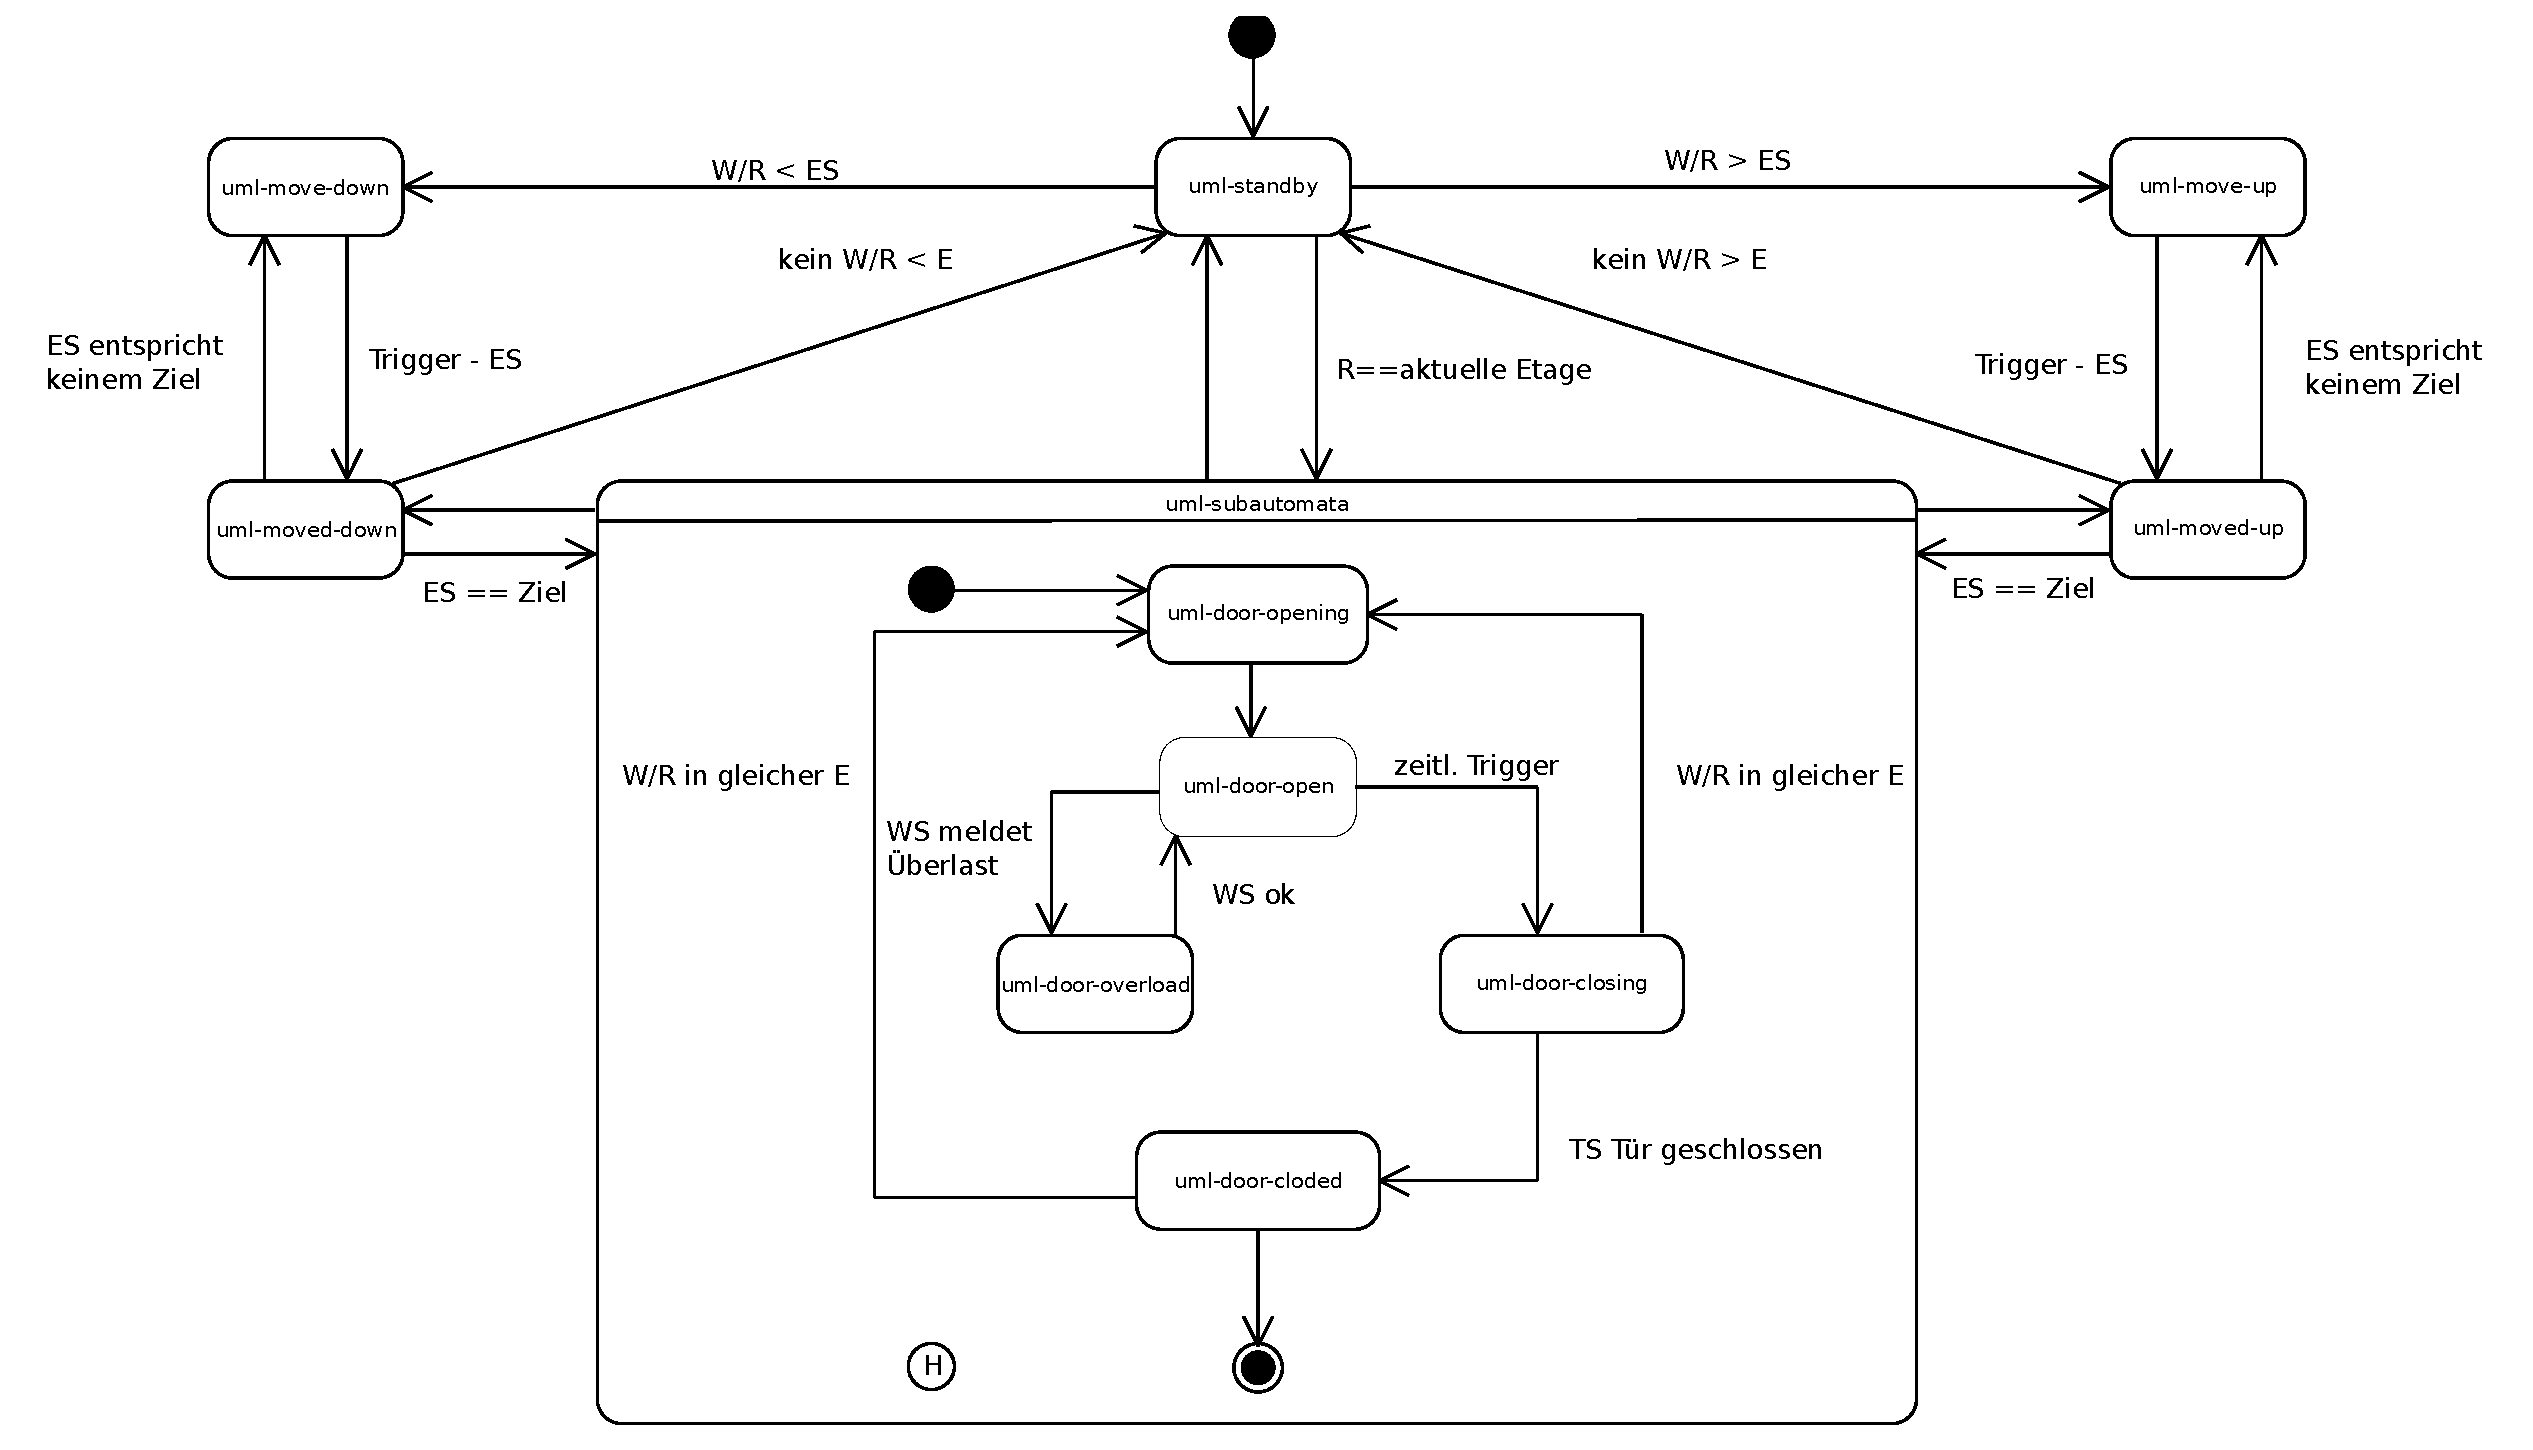
\includegraphics[width=\textwidth]{images/ZDv6_id_view.eps}
\caption{IDs des Zustandsdiagrammes}%
\label{fig:ZD_id_view}%
\end{figure}
\chapter{Klassendiagramme}
\chapter{API}
\chapter{Build-Prozess}
